\appendix{Представление графического материала}

Графический материал, выполненный на отдельных листах,
изображен на рисунках А.1--А.\arabic{числоПлакатов}.
\setcounter{числоПлакатов}{0}

\renewcommand{\thefigure}{А.\arabic{figure}} % шаблон номера для плакатов

\begin{landscape}

\begin{плакат}
	
\includegraphics[width=0.82\linewidth,page=1]{plac1.eps}
	\заголовок{Сведения о ВКРБ}
	\label{plac1:image}      
\end{плакат}

\begin{плакат}
	\includegraphics[width=0.82\linewidth,page=2]{plac2.eps}
	\заголовок{Цели и задачи разработки}
	\label{plac2:image}      
\end{плакат}


\begin{плакат}
	\includegraphics[width=0.82\linewidth,page=3]{plac3.eps}
	\заголовок{Диаграмма прецедентов}
	\label{plac3:image}      
\end{плакат}


\begin{плакат}
	
\includegraphics[width=0.82\linewidth,page=4]{plac4.eps}
	\заголовок{Архитектура приложения}
	\label{plac4:image}      
\end{плакат}


\begin{плакат}
	\includegraphics[width=0.82\linewidth,page=5]{plac5.eps}
	\заголовок{Интерфейс программы}
	\label{plac5:image}      
\end{плакат}


\begin{плакат}
	\includegraphics[width=0.82\linewidth,page=6]{plac6.eps}
	\заголовок{Интерфейс вкладки компрессора и графиков}
	\label{plac6:image}      
\end{плакат}


\begin{плакат}
	\includegraphics[width=0.82\linewidth,page=7]{plac7.eps}
	\заголовок{Интерфейс вкладки реверберации и графиков}
	\label{plac7:image}      
\end{плакат}

\begin{плакат}
	
\includegraphics[width=0.82\linewidth,page=8]{plac8.eps}
	\заголовок{Заключение}
	\label{plac8:image}      
\end{плакат}

\end{landscape}
